Consider the following feedback control system.
\begin{center}
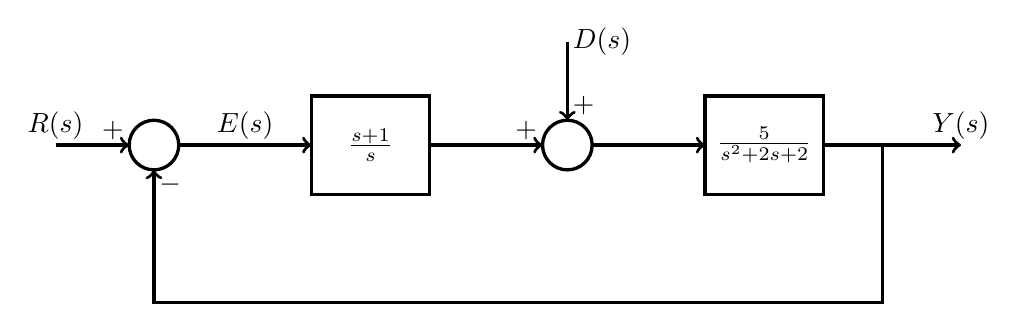
\begin{tikzpicture}[scale=1,inner sep=0pt,outer sep=0pt,very thick,
sysblock/.style={draw,rectangle,inner sep=2pt,minimum width=1.5cm,minimum height=1.25cm,very thick}]

\draw (1.25,0) node[draw,circle] (sum1) {$\rule{0pt}{18pt}$};
\draw (4,0) node[sysblock] (Kp) {$\frac{s+1}{s}$};
\draw (6.5,0) node[draw,circle] (sum2) {$\rule{0pt}{18pt}$};
\draw (9,0) node[sysblock] (G) {$\frac{5}{s^2+2s+2}$};

\draw[->] (0,0) node[above=2pt] {$R(s)$} -- (sum1.180) node[above left=2pt] {$+$};
\draw[->] (sum1.0) --  node[above=2pt,pos=.5] {$E(s)$} (Kp);
\draw[->] (Kp) --  (sum2.180) node[above left=2pt] {$+$};
\draw[->] (sum2.0) -- (G);
\draw[->] (G) -- ++(2.5,0) node[above=2pt] {$Y(s)$};
\draw[->] (G) ++(1.5,0) -- ++(0,-2) -| (sum1.-90) node[below right=2pt] {$-$};
\draw[<-] (sum2.90) node[above right=2pt] {$+$} -- ++(0,1) node[right=2pt] {$D(s)$};
\end{tikzpicture}
\end{center}
\begin{enumerate}[(a)]
\item Use the Routh-Hurwitz criterion to show that the closed loop system is stable.
\item If $r(t)=t$ (unit ramp) and $d(t)=0$ for $t\geq 0$, is $\lim_{t\rightarrow\infty}e(t)=0$?
\item If $r(t)=0$ and $d(t)=2$ (step of magnitude 2) for $t\geq 0$  what is $\lim_{t\rightarrow \infty} y(t)$?
\end{enumerate}


